\section{Evaluation}
\label{sec:eval}

We've evaluated Tutamen in a variety of scenarios. These scenarios
have proven Tutamen's usefulness as an enabler of previously
unattainable functionally and use cases. While Tutamen is still a
prototype, we feel it provides a well designed architecture capable of
supporting a wide range of practical secret storage applications.

\subsection{Server Performance}

Our Tutamen reference implementation provides a usable prototype with
which to experiment with Tutamen applications. While the server
software has not yet been optimized for performance, we have performed
a number of performance measurements in order to better understand the
computational load a system like Tutamen requires.

\begin{figure}[th]
  \centering
  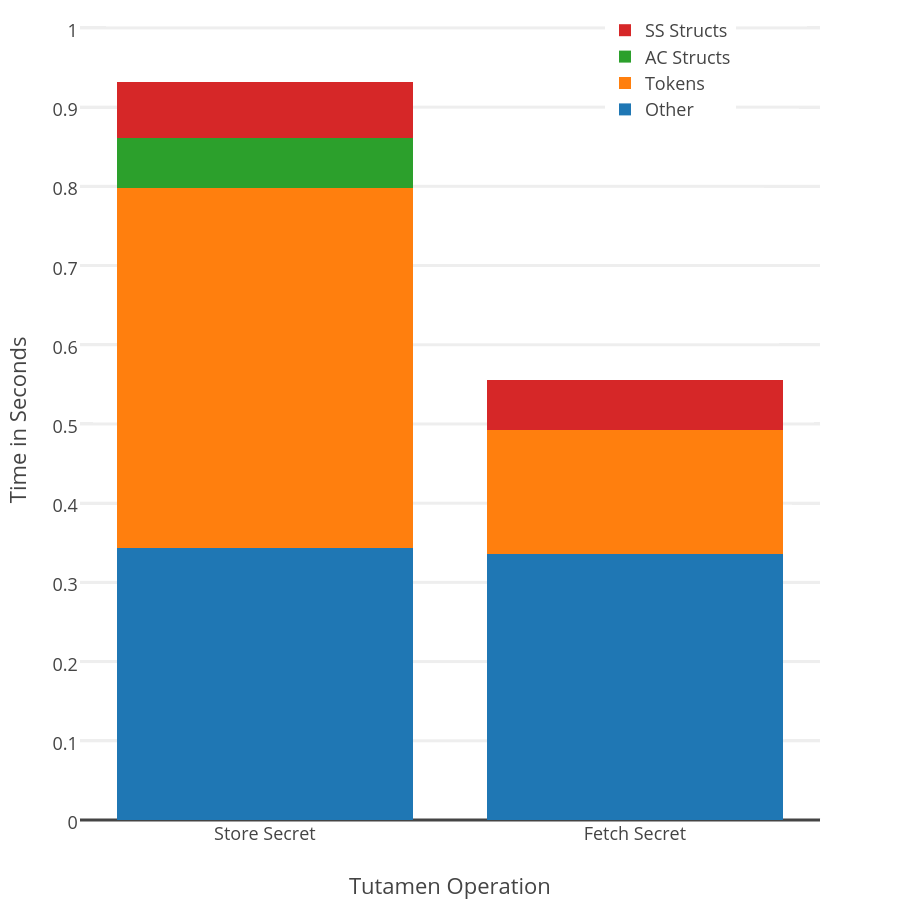
\includegraphics[width=\columnwidth]{./figs/png/chart-combined-timings.png}
  \caption{Timings for Tutamen Operations}
  \label{fig:eval:timings}
\end{figure}

Figure~\ref{fig:eval:timings} shows the time required to complete two
of the most common Tutamen operations: storing a new secret and
retrieving a previously stored secret. We measured the amount to time
the Tutamen CLI application spent performing various parts of each of
these two Tutamen operations. In both operations, the bulk of the
server-related run time is spent requesting and retrieving the
authorization tokens required to complete the associated
operations. In the secret creation case, five tokens are
required\footnote{Two permission group creation tokens (one for the
  collection permission group and one for the verifier itself), one
  verifier creation token, one collection creation token, and one
  secret creation token.}. In the secret read case only a single token
is required\footnote{The collection read permission token}. The
reminder of the server-related time is spent either creating AC and
storage data structures (as in the store secret case) or reading
existing data structures (as in the retrieve secret case). The
``other'' time is spent reading the Tutamen config files, loading the
necessary client certificates, and dealing with the overhead required
to interpret the python-based CLI.

It is not unexpected that the client must spend the bulk of its time
requesting tokens and waiting for them to be approved -- token
verification is the primary role the access control server must
perform, and depending on the complexity of the verifiers associated
with the permission the token is requesting, verification can be a
fairly complex task. When performing these measurements, we employed a
simple verifier that only required client membership in a specific
account. Verifiers that include human-in-the-loop authenticators
(e.g. SMS approval) would increase the token turnaround time by the
amount of time the human requires to provide approval. Thus, it's
important that Tutamen applications treat token approval as an
operation that can take anywhere from under a second to 10s of
seconds. To help alleviate these waits on applications that must
perform a high number of Tutamen requests, our deign allows Tutamen
tokens to be reused up until their expiration time. Thus, its possible
for an applications to request a long lived token\footnote{Token
  expiration time is included in data presented to each authenticator
  module -- it's thus possible for these modules to factor the token
  length into their decisions regrading whether or not to approve the
  token request. This is useful in cases where a module wishes to
  require a higher level of confidence in the validity of a request
  for long-lived tokens.} and to reuse this same token to access
e.g. multiple secrets within the collection to which the token grants
read access.
 
\begin{figure}[th]
  \centering
  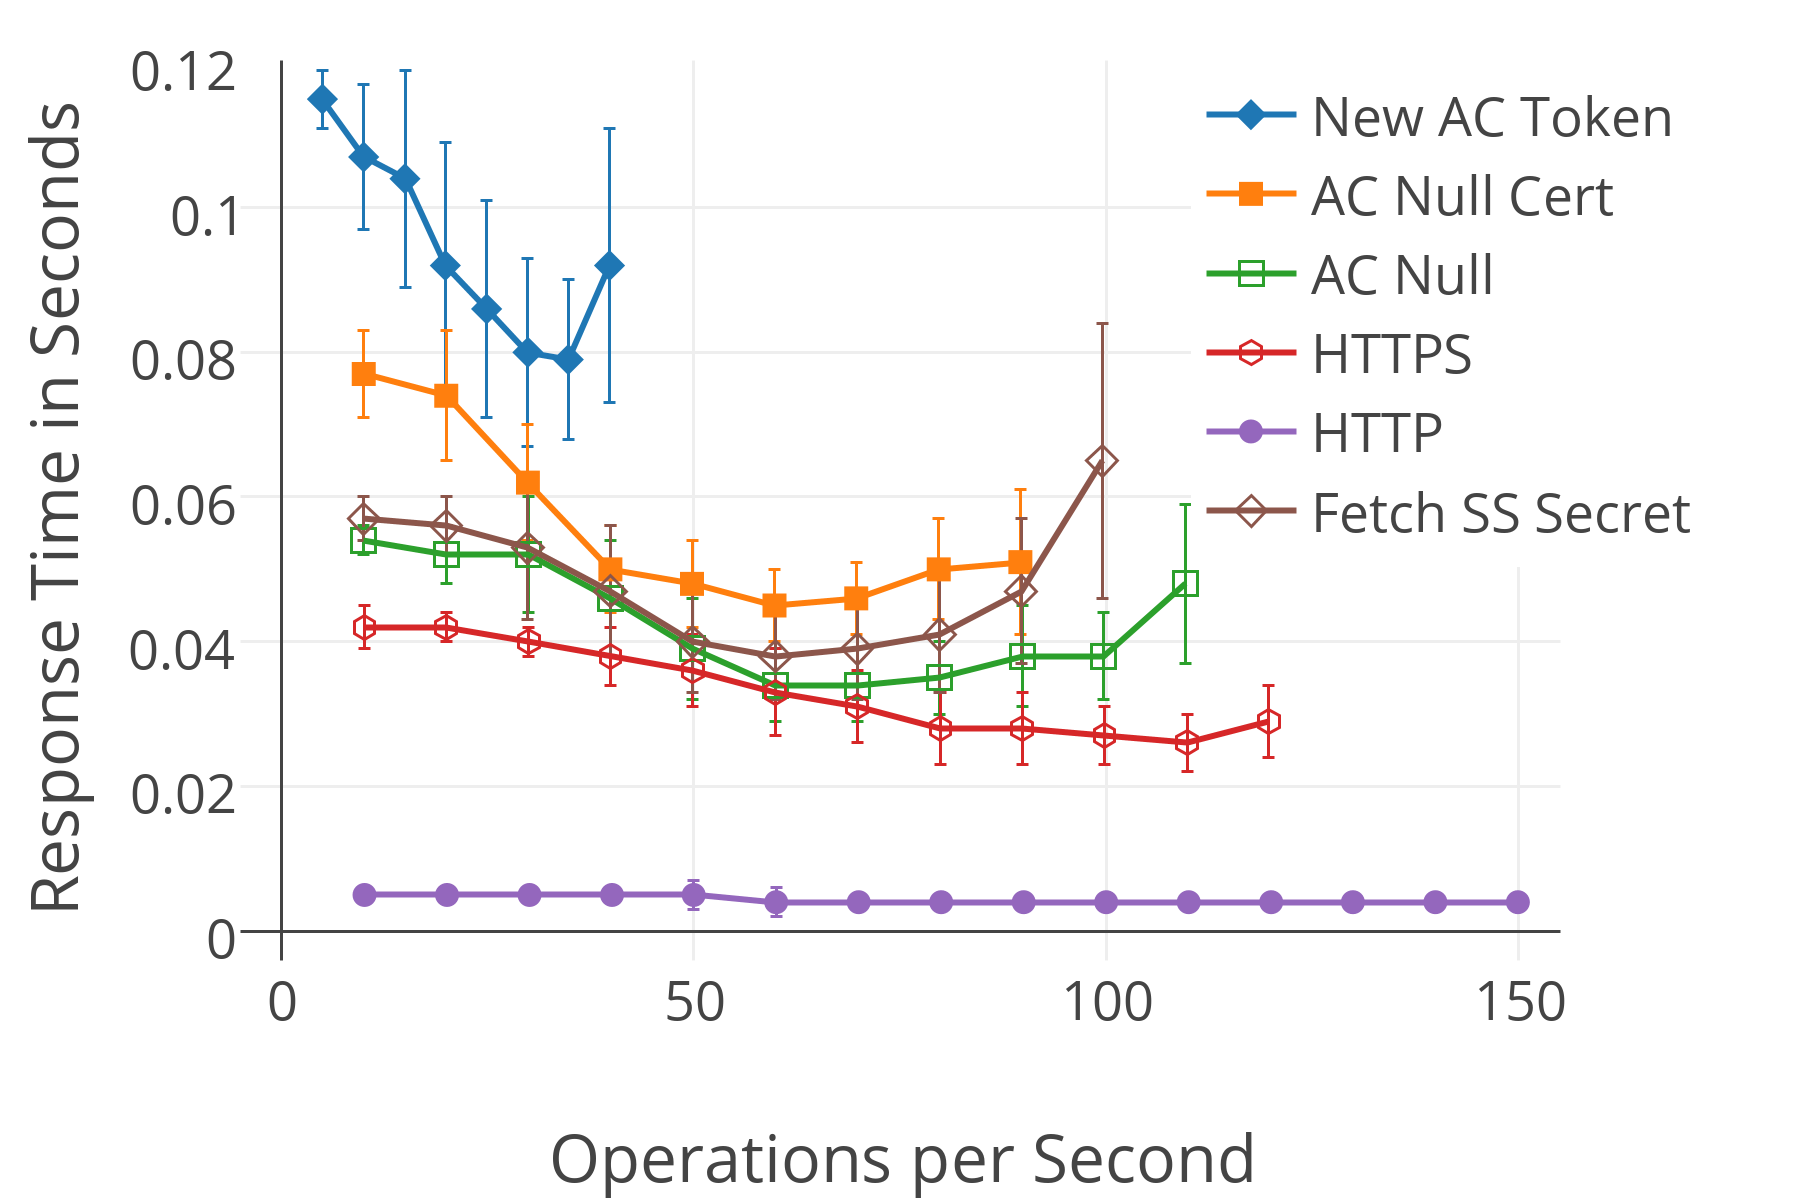
\includegraphics[width=\columnwidth]{./figs/png/chart-iops.png}
  \caption{Throughput vs Latency}
  \label{fig:eval:iops}
\end{figure}

Figure~\ref{fig:eval:iops} shows the request rate vs response time
(with standard deviations) of a single access control server for both
the token request operation as well as for two ``null'' operations:
one which loads a simple ``Hello'' message (but that still verifies
the client TLS certificate required to perform most Tutamen AC server
operations) and one which loads the same message but without providing
or verifying client certificates. As these curves show, token
verification of our prototype server tops out at around 40
requests/second on moderate hardware (e.g. a 4-core, 4GB VM running
atop 2011-era Intel Xeon hardware). The null operation with client
certificates top out around 60 requests per second and the null
operation itself tops out at about 70 request per second. The current
server setup is thus primarily limited by the TLS and WSGI overhead
required to serve the application. Token verification itself does
ensure additional computational requirements - largely limited by the
database speed required to provide access to all of the necessary data
structures that must be inspected in order to evaluate the validity of
a given token request.

% Todo: Storage server curves?

While these levels of performance would not likely meet the
requirements of a production-level Tutamen AC server, they have been
perfect adequate for our needs and have been cable of supporting the
handful of Tutamen applications we're currently using. Since must of
our Tutamen applications require only a single Tutamen secret
retrieval at relatively rare rates (e.g. once per server reboot, or
once per file open) the 30-40 requests per second or server can
provide have been more than adequate for our needs. We've also
designed our reference server to be horizontally scalable in both its
HTTPS request handling (e.g. by spinning up multiple load-balanced
front-end servers each ruining their own Apache WSGI instance) as well
as in its backing database (Redis is capable of distribution across
multiple systems). That scalability, couple with future
performance-related code optimization lead us to believe the Tutamen
server infrastructure can be adopted to meet the needs of larger
installations with only moderate effort.

\subsection{Usage}

Maybe move the usefulness of the various application discussion to
here? Otherwise, this should probably just be the ``Performance''
section, not the ``Evaluation'' section...

%%  LocalWords:  Tutamen Tutamen's verifiers authenticators SMS Xeon
%%  LocalWords:  authenticator HTTPS Redis
